\documentclass[a4paper]{ctexart}
\usepackage[top=2.3cm,bottom=2cm,left=1.7cm,right=1.7cm]{geometry} 
\usepackage{amsmath, amssymb}
\usepackage{color}
\usepackage{listings}
\usepackage{mathrsfs} 
\usepackage{booktabs}
\usepackage{amsthm}
\usepackage{longtable} 
\usepackage{graphicx}
\usepackage{subfigure}
\usepackage{caption}
\usepackage{fontspec}
\usepackage{titlesec}
\usepackage{fancyhdr}
\usepackage{latexsym}
\usepackage{subfigure}
\CTEXsetup[format={\Large\bfseries}]{section}
\def\d{\mathrm{d}}
\def\e{\mathrm{e}}
\newcommand{\mb}[1]{\mathbf{#1}}
\newcommand{\mr}[1]{\mathrm{#1}}
\newcommand{\dv}[2]{\frac{\d{#1}}{\d{#2}}}
\newcommand{\pdv}[2]{\frac{\partial{#1}}{\partial{#2}}}
\def\degree{$^{\circ}$}
\title{\textbf{鼓的振动模态}}
\author{王崇斌\;1800011716}
\date{}

\makeatletter %使\section中的内容左对齐
\makeatother
\begin{document}
	\pagestyle{fancy}
	\pagestyle{fancy}
    \lhead{音乐与数学期末课题}
	\chead{}
	\rhead{\today}
	\maketitle
	\thispagestyle{fancy}
	\section{鼓与振动}
	\subsection{鼓的构造}
	鼓是一种由近似圆柱形的鼓身和鼓身一端或两端蒙上拉紧的膜构成的打击乐器。
	演奏时通常是演奏者击打圆形的鼓面,鼓面振动发出声音,可以将发声过程看作
	圆形薄膜的振动过程。但是真实的鼓发声过程并不简单地对应于一个边界固定的
	圆形薄膜的自由振动(没有耗散,没有外力),比如我们忽略了鼓面的能量耗散:
	鼓面与空气的相互作用,鼓面本身的阻尼等等。想要建立准确的符合实际的模型,
	首先需要在物理上对鼓进行分类。
	\par 鼓作为振动系统可以分为3类[1]:
	1.由单个薄膜与封闭的空气室构成(kettledrums),2.由单个薄膜和两侧均开放的空气室构成(tom-toms, congas),
	3.由两片薄膜与中间封闭的空气室耦合而成(bass drums, snare drums)。可以看到,
	真实的情况远比理想的薄膜振动要复杂,不仅涉及到鼓面与空气作用导致的能量耗散,甚至
	涉及到两个鼓面振动的耦合。
	\subsection{膜自由振动波动方程的建立}
	要想精确描述一个振动过程,必须找到与之对应的波动方程。但是真实的情况非常复杂,
	只能先从理想的情况开始讨论。
	我们\textbf{假设}膜上的每一点都在垂直于薄膜平面(平衡位置)的方向上做小振动,
	这样用一个标量可以完全描述每一点的运动情况,得到的波动方程是标量波动方程。
	用坐标$(x, y)$来标记平衡时每一点的位置,用$u(x, y)$来标记与平衡位置的偏离。
	\textbf{假设}薄膜没有厚度,薄膜的形变不能带来法向的张力,
	即膜的内部只有平行于薄膜的张力(这个假设与柔软的弦是一样的),
	很显然这个假设对于平板(和细杆)是不成立的,也就是说将要得到的波动方程
	并不能描述与它们的振动。
	\par 建立波动方程的思路是考虑一小块薄膜的受力情况,写出它对应的运动方程。如下图
	所示,OABC表示偏离平衡位置的薄膜,O点的坐标为$(x, y)$。假设这个薄膜的应力张量
	为$\sigma$,在最一般的情况下也是位置与时间的函数。
	\begin{figure}[htbp]
		\centering
		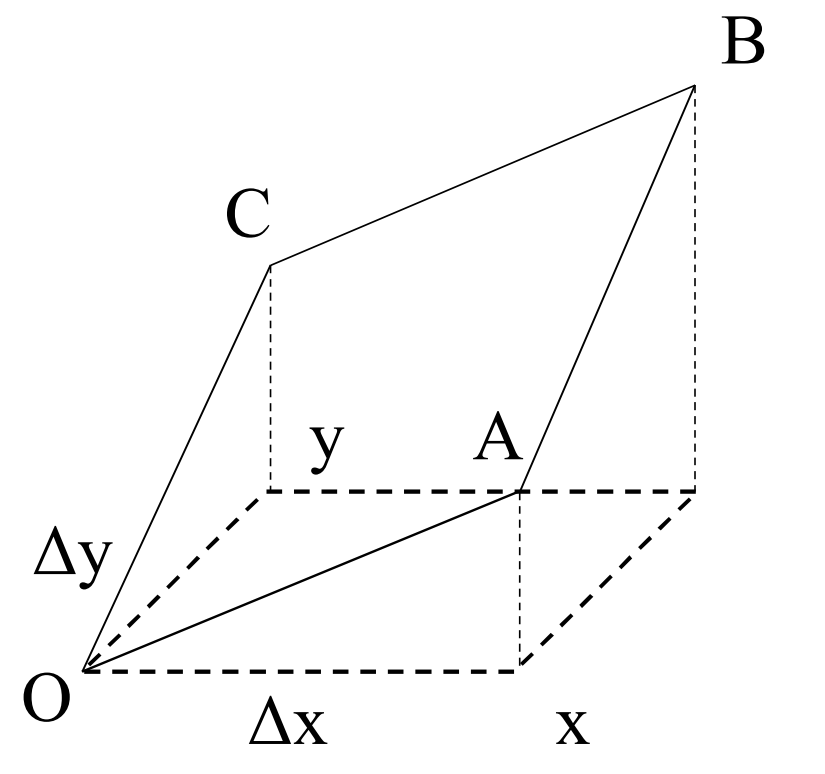
\includegraphics[scale=0.2]{force.png}
		\caption{受力分析}
	\end{figure} 
	可以通过应力张量表示出这个小薄膜的每个边的受力情况:
	\begin{align}
		F_{\mr{AB}, x} &= \int_{\mr{A}}^{\mr{B}} \sigma_{xy}\d x + \sigma_{xx}\d y \approx \sigma_{xx}(x+\Delta x, y)\Delta y\\
		F_{\mr{AB}, y} &= \int_{\mr{A}}^{\mr{B}} \sigma_{yy}\d x + \sigma_{yx}\d y \approx \sigma_{yx}(x+\Delta x, y)\Delta y\\
		F_{\mr{OC}, x} &= \int_{\mr{O}}^{\mr{C}} \sigma_{xy}\d x + \sigma_{xx}\d y \approx \sigma_{xx}(x, y)\Delta y\\
		F_{\mr{OC}, y} &= \int_{\mr{O}}^{\mr{C}} \sigma_{yy}\d x + \sigma_{yx}\d y \approx \sigma_{yx}(x, y)\Delta y\\
		F_{\mr{OA}, x} &= \int_{\mr{O}}^{\mr{A}} \sigma_{xy}\d x + \sigma_{xx}\d y \approx \sigma_{xy}(x, y)\Delta x\\
		F_{\mr{OA}, y} &= \int_{\mr{O}}^{\mr{A}} \sigma_{yy}\d x + \sigma_{yx}\d y \approx \sigma_{yy}(x, y)\Delta x\\
		F_{\mr{CB}, x} &= \int_{\mr{C}}^{\mr{B}} \sigma_{xy}\d x + \sigma_{xx}\d y \approx \sigma_{xy}(x, y + \Delta y)\Delta x\\
		F_{\mr{CB}, y} &= \int_{\mr{C}}^{\mr{B}} \sigma_{yy}\d x + \sigma_{yx}\d y \approx \sigma_{yy}(x, y + \Delta y)\Delta x
	\end{align}
	\par 上面的约等于在薄膜很小的情况下成立,忽略了一些在后面计算二阶导数时可以忽略的高阶小量。
	下面将计算每个边的受力在$z$方向上的分量(因为我们假设只在$z$方向上有运动),
	\textbf{假设}薄膜只做微小的振动,在这种情况下,$x$方向的力在$z$方向的贡献可以用
	薄膜沿$x$方向的切线与$x$轴夹角的正切值,也就是$\pdv{u}{x}$来衡量;同样的,$y$方向的
	力对$z$方向的力的贡献可以用$\pdv{u}{y}$来衡量。那么AB,\, CO两个边对于$z$方向的力的
	贡献为:
	\begin{align}
		F_{1} =& \,\sigma_{xx}(x+\Delta x, y)\Delta y\pdv{u}{x}(x+\Delta x, y) + \sigma_{yx}(x+\Delta x, y)\Delta y\pdv{u}{y}(x+\Delta x, y)\\
		&- \sigma_{xx}(x, y)\Delta y\pdv{u}{x}(x, y) + \sigma_{yx}(x, y)\Delta y\pdv{u}{y}(x, y)\\
		\approx& \, \left[\pdv{}{x}\left(\sigma_{xx}\pdv{u}{x}\right) + \pdv{}{x}\left(\sigma_{yx}\pdv{u}{y}\right)\right]\Delta x\Delta y
	\end{align}
	\par 同理OA,\, CB两个边对于$z$方向力的贡献为:
	\begin{align}
		F_{2} \approx  \left[\pdv{}{y}\left(\sigma_{xy}\pdv{u}{x}\right) + \pdv{}{y}\left(\sigma_{yy}\pdv{u}{y}\right)\right]\Delta x\Delta y
	\end{align}
	\par 那么,根据Newton运动定律,薄膜微元的振动方程可以写为:
	\begin{align}
		&F_{1} + F_{2} = \rho \Delta x\Delta y \pdv{^{2}u}{t^{2}}\\
		\Rightarrow& \left[\pdv{}{x}\left(\sigma_{xx}\pdv{u}{x}\right) + \pdv{}{x}\left(\sigma_{yx}\pdv{u}{y}\right)\right] + 
		\left[\pdv{}{y}\left(\sigma_{xy}\pdv{u}{x}\right) + \pdv{}{y}\left(\sigma_{yy}\pdv{u}{y}\right)\right] = \rho\pdv{^2 u}{t^{2}}
	\end{align}
	\par 这是一般的没有能量耗散的薄膜小振动时所满足的方程,其中应力张量可以是位置
	和时间的函数,在小振动假设下,一般认为其只是位置的函数。考虑到应力张量总是一
	个对称张量[2],可以将上面的波动方程表示为一个更加紧凑的形式,其中使用了求和约定:
	\begin{align}
		\pdv{}{x^{i}}\left(\sigma_{ij}\pdv{u}{x^{j}}\right) = \rho\pdv{^2 u}{t^2}
	\end{align}
	
	进一步\textbf{假设}薄膜在平衡时内部的应力张量是一个常量(与位置无关,比如在各个
	方向均匀地拉伸一个各向同性方形薄膜),同时考虑到这是一个对称张量,那么可以选取
	一个特殊的直角坐标系使得每一点处的张量都具有对角的形式,方程可以化简为:
	\begin{align}
		\sigma_{xx}\pdv{^{2}u}{x^{2}} + \sigma_{yy}\pdv{^2 u}{y^2} = \rho \pdv{^{2}u}{t^{2}}
	\end{align}
	\par 如果进一步假设薄膜是各向同性的,应力张量为一个常数乘上单位张量
	那么薄膜的小振动方程在任意一个直角坐标系下都可以写成:
	\begin{align}
		\pdv{^2 u}{x^2} + \pdv{^{2}u}{y^{2}} = \frac{1}{c^{2}}\pdv{^2 u}{t^2}\quad\quad\quad c^2 = \frac{\rho}{\sigma}
	\end{align}
	\par 其中$c$称为波速。将要求解的就是这个波动方程,这是一个理想化的模型,我们做了足够多的假设。
	\section{固定边界的圆膜自由振动}
	\subsection{问题的描述}
	由于鼓面的四周是完全固定的,在考虑初始条件后可以构成一个定解问题。假设
	圆膜的半径为$a$,给定初始时刻时圆膜上每一点的位移和速度,定解问题可以写为:
	\begin{align}
		\left\{
			\begin{array}{lr}
				\frac{1}{c^2}\pdv{^{2}u}{t^2} = \nabla^{2}u\\
				u|_{x^2 + y^2 = a^2} = 0\\
				u|_{t=0} = f(x, y),\, \pdv{u}{t}|_{t=0} = g(x, y)
			\end{array}
		\right.
	\end{align}
	\par 由于求解区域的特殊性,考虑将方程转化到极坐标中,同时要转换方程与定解条件:
	\begin{align}
		\left\{
			\begin{array}{lr}
				\frac{1}{c^2}\pdv{^{2}u}{t^2} = \frac{1}{r}\pdv{}{r}\left(r\pdv{u}{r}\right) + \frac{1}{r^2}\pdv{^2 u}{\phi^{2}}\\
				u|_{\phi=0} = u|_{\phi=2\pi},\, \pdv{u}{\phi}|_{\phi=0} = \pdv{u}{\phi}|_{\phi=2\pi}\\
				u|_{r=0}\,\mr{finit},\, u|_{r=a}=0\\
				u|_{t=0} = F(r, \phi),\, \pdv{u}{t}|_{t=0} = G(r, \phi)
			\end{array}
		\right.
	\end{align}
	\par 注意到将直角坐标转换成极坐标时,人为地增添了一些边界条件,这些边界条
	件在物理上很好理解:首先在直角坐标系中原点并不是奇点,因此转换为极坐标后我们
	也得要求原点的解不能发散(不是奇点);其次这个解应该是角度的周期函数,
	因为转过$2\pi$角度后回到圆膜上同一个点,同一个点的振动是完全相同的。
	\par 也可以给出直观上的从数学角度的理解(个人的理解,其中可能包含不严谨
	的语言):直角坐标与极坐标之间的变换将一个圆形和一个长方形对应了起来,
	但是这个“对应”的性质并不总是很好,首先圆心处映射并不是单射,圆心对应于
	长方形的一个边;其次边界并不对应边界,圆形的边界对应于长方形的一个边,
	圆形区域内部的一条线(规定$\phi=0$的那条线)对应于长方形的两个边。
	这个映射破坏了原本圆形的拓扑,相当于挖去了圆心后再沿圆心处将圆形剪开,
	再把这个图形“连续地”映射成了一个长方形。在计算积分时,由于“性质不好”的点
	对于积分的贡献为零,所以可以使用这个变换计算积分。但是讨论区域上的函数时,
	区域的性质会影响其上函数的性质,最直接的就是影响连续性和可微性,上面的边界条件
	相当于将定义在矩形上的函数“沿着某个边粘起来”,使之可以定义在圆形的区域上。
	\par 我们将要求解的是这个转化到极坐标后,与原来问题等价的方程。
	\subsection{没有耗散的情形}
	上面导出的方程就对应于没有耗散的情形。首先假设方程具有满足$r\, \phi$方向
	边界条件(不一定满足初始条件)的分离变量形式的特解:
	\begin{align}
		u(r, \phi, t) = v(r, \phi)T(t)
	\end{align}
	将上面这样形式的解线性组合使得其满足初始条件就可以得到定解问题的解。
	将上面形式的解代入方程:
	\begin{align}
		\frac{1}{c^2}\frac{T^{''(t)}}{T} = \frac{1}{rv(r,\phi)}\pdv{}{r}\left(r\pdv{v}{r}\right)
		 + \frac{1}{r^2 v(r,\phi)}\pdv{^2 V}{\phi^2}
	\end{align}
	方程两边没有相同的自变量因此只能等于一个常数,令其为$k^2$,得到两个方程:
	\begin{align}
		\left\{

		\right.
	\end{align}
	\subsection{有阻尼的情形}
	\section{定音鼓的发声机制}
	\section{有固定音高乐器与无固定音高乐器}
	\begin{thebibliography}{99}
		\bibitem{ref1}Neville H. Fletcher, Thomas D. Rossing, The physics of musical instruments, Springer-Verlag, New York, 1991, 第18章.
		\bibitem{ref2}理论物理学教程第七卷\,弹性理论(第五版)朗道\, 栗弗席茨\,第一章第二节
	\end{thebibliography}
\end{document}
